\documentclass[ignorenonframetext, professionalfonts, hyperref={pdftex, unicode}]{beamer}
%\usepackage{beamerthemesplit}

\geometry{paperwidth=140mm,paperheight=105mm}

%Hack to specify beamer folder https://tex.stackexchange.com/questions/275600/beamer-themes-on-custom-folder
\makeatletter
  \def\beamer@calltheme#1#2#3{%
    \def\beamer@themelist{#2}
    \@for\beamer@themename:=\beamer@themelist\do
    {\usepackage[{#1}]{\beamer@themelocation/#3\beamer@themename}}}

  \def\usefolder#1{
    \def\beamer@themelocation{#1}
  }
  \def\beamer@themelocation{}
\makeatother
%Packages to be included

\usepackage{graphicx}



\graphicspath{{./branding/}}
\usefolder{./branding}
\usetheme{Promwad}
%\usecolortheme{wolverine}


\usepackage[russian]{babel}
\usepackage[utf8]{inputenc}
\usepackage[T1]{fontenc}

%\usepackage[orientation=landscape, size=custom, width=16, height=9, scale=0.5]{beamerposter}

\usepackage{textcomp}


\usepackage{ulem}

\usepackage{verbatim}

\usepackage{ucs}


\usepackage{listings}
\lstloadlanguages{bash}

\lstset{escapechar=`,
	extendedchars=false,
	language=sh,
	frame=single,
	tabsize=2, 
	columns=fullflexible, 
%	basicstyle=\scriptsize,
	keywordstyle=\color{blue}, 
	commentstyle=\itshape\color{brown},
%	identifierstyle=\ttfamily, 
	stringstyle=\mdseries\color{green}, 
	showstringspaces=false, 
	numbers=none, 
%	numberstyle=\tiny, 
	breaklines=true, 
	inputencoding=utf8,
	keepspaces=true,
	morekeywords={u\_short, u\_char, u\_long, in\_addr}
	}

\definecolor{darkgreen}{cmyk}{0.7, 0, 1, 0.5}

\lstdefinelanguage{diff}
{
    morekeywords={+, -},
    sensitive=false,
    morecomment=[l]{//},
    morecomment=[s]{/*}{*/},
    morecomment=[l][\color{darkgreen}]{+},
    morecomment=[l][\color{red}]{-},
    morestring=[b]",
}

\author[Promwad]{{\bf Promwad}}

%\institution[EPAM]{EPAM}
%\logo{\includegraphics[width=1cm]{logo.png}}

\AtBeginSection[]{%
  \begin{frame}<beamer>
    \frametitle{}
    \tableofcontents[
        sectionstyle=show/shaded, hideallsubsections ]
  \end{frame}
  \addtocounter{framenumber}{-1}% If you don't want them to affect the slide number
}

\AtBeginSubsection[]{%
  \begin{frame}<beamer>
    \frametitle{}
    \tableofcontents[
        sectionstyle=show/hide,
        subsectionstyle=show/shaded/hide, ]
  \end{frame}
  \addtocounter{framenumber}{-1}% If you don't want them to affect the slide number
}

\title{Сборка дистрибутивов для embedded}

\begin{document}

\begin{frame}
  \frametitle{}
  \titlepage
\end{frame}

\section{Ручная сборка дистрибутива}

\subsection{Компоненты дистрибутива}
\begin{frame}
  \frametitle{Основные части загрузочного образа}
  \begin{itemize}
    \item{Загрузчик}
    \item{Ядро}
    \item{Образ файловой системы с ПО}
      \begin{itemize}
        \item Минимальный образ: busybox с /sbin/init shell скриптом
      \end{itemize}
  \end{itemize}
\end{frame}

\subsection{Лирическое отступление: порядок загрузки}

\begin{frame}
  \frametitle{Порядок загрузки стандартной системы на arm}
\end{frame}

\begin{frame}
  \frametitle{Порядок загрузки raspberry pi}
  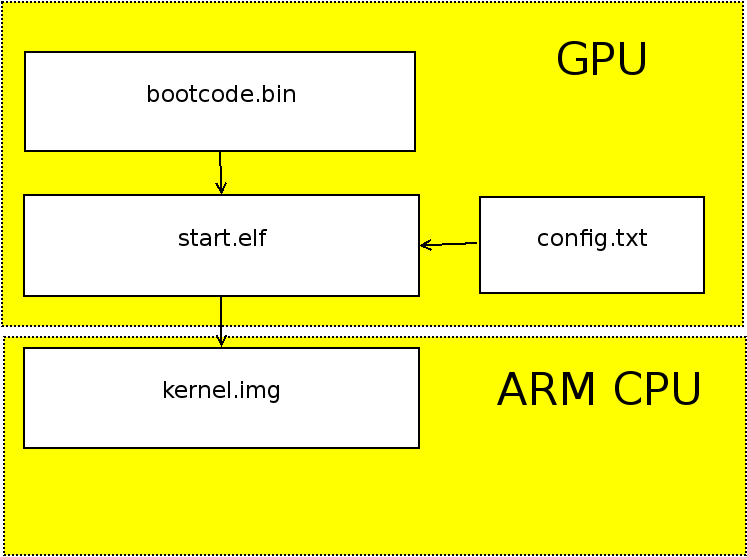
\includegraphics[height=6cm]{rpi_boot.png}
\end{frame}

\subsection{Порядок сборки дистрибутива}

\begin{frame}
  \frametitle{}
  \begin{itemize}
      \item Добыча кросс-компилятора
      \item Выбор и сборка стандартной библиотеки (иногда вместе с компилятором)
      \item Компиляция u-boot
      \item Компиляция ядра (и получение хедеров)
      \item Компиляция busybox
      \item Компиляция прикладных программ
      \item Сборка образа прошивки
  \end{itemize}
\end{frame}

\begin{frame}
  \frametitle{Где брать компиляторы}
  \begin{itemize}
    \item Свой дистрибутив (Debian: gcc-arm-linux-gnueabi )
    \item Linaro \url{https://www.linaro.org/downloads/}
    \item crosstool-ng \url{http://crosstool-ng.org/}
    \item Ручная компиляция из исходников \url{http://clfs.org/view/clfs-embedded/arm/cross-tools/chapter.html}
    \item Codesourcery (deprecated)
  \end{itemize}
\end{frame}

\begin{frame}
  \frametitle{Опции для стандартной библиотеки}
  \begin{itemize}
      \item glibc - \url{http://www.gnu.org/software/libc/} самая большая
      \item uClibc -\url{http://uclibc-ng.org/}
      \item musl - \url{http://www.musl-libc.org/}
      \item dietlibc - \url{http://fefe.de/dietlibc/} 
      \item newlib - \url{http://sourceware.org/newlib/}
  \end{itemize}
\end{frame}

\subsection{Cборка u-boot}

\begin{frame}
  \frametitle{Система kconfig/kbuild}
  \begin{itemize}
      \item Изначально: система конфигурации и сборки ядра
      \item В настоящее время: ядро, buildroot, busybox, u-boot, ...
      \item Основана на makefilах
      \item Дополнительные утилиты: mconf, lxdialog, etc.
  \end{itemize}
\end{frame}

\begin{frame}[fragile]
  \frametitle{Упражнение}
  \begin{itemize}
    \item Распаковать \texttt{sample-packages.tgz}
    \item Распаковать linaro toolchain
    \item \verb+export CCPREFIX=<path to linaro>/bin/arm-linux-gnueabihf- +
    \item Найти файл mconf.c среди файлов в директории u-boot
    \item Посмотреть на содержимое директории configs (в директории u-boot)
    \item Найти все файлы с именем Kconfig и посмотреть на их содержание
  \end{itemize}

\end{frame}

\begin{frame}[fragile]
  \frametitle{Продолжение упражнения}
  \begin{itemize}
    \item \verb+ARCH=arm CROSS_COMPILE=${CCPREFIX} make rpi_3_32b_defconfig +
    \item \verb+ARCH=arm CROSS_COMPILE=${CCPREFIX} make menuconfig +
    \item Найти опцию \verb+ BOOTDELAY +
    \item Установить BOOTDELAY в 10 секунд
    \item Собрать u-boot
  \end{itemize}
\end{frame}

\subsection{Работа с u-boot}

\begin{frame}[fragile]
  \frametitle{Установка на карточку}
  \begin{itemize}
      \item Распаковать debian-lite 
      \item ОПАСНОСТЕ! \verb+dd if=<img file> of=/dev/<card device> + 
      \item Смонтировать первый раздел карточки
      \item Добавить \verb+ enable_uart=1 + в config.txt
      \item Скопировать u-boot.bin на этот раздел
      \item Отредактировать config.txt заменить kernel.img на u-boot.bin
  \end{itemize}
\end{frame}

%\begin{frame}[fragile]
%  \frametitle{Возимся с u-boot}
%\end{frame}

\begin{frame}[fragile]
  \frametitle{Пытаемся загрузиться}
\begin{lstlisting}[language=bash]
fatload mmc 0:1 ${kernel_addr_r} kernel7.img+ 
fatload mmc 0:1 0x2000000 bcm2710-rpi-3-b.dtb +
setenv bootargs 8250.nr_uarts=1 root=/dev/mmcblk0p2 rootwait console=ttyS0,115200 +
bootz ${kernel_addr_r} - 0x2000000 +
\end{lstlisting}
\end{frame}

\end{document}
